\documentclass{article}
\usepackage[utf8]{inputenc}
\usepackage[english]{babel}
\usepackage{biblatex}
\usepackage{graphicx}
\addbibresource{completedCILib.bib}

\begin{document}
\tableofcontents
\newpage
\section{Introduction}
Responsible code development is not a byproduct of good programmers.
It is a paradigm of development in and of itself. It is this paradigm that shapes
the modern programmer, the weight on which it lays can be seen in the software issues of the past.
The Therac-25, was a machine with software that had not been scrutinized, leading to deaths. The 2012 Knight Capital incident
led to losses of millions because of issues stemming from integrating changes into an old system. The Y2K incident
spread panic among civilians based on the idea that the internal clocks of old systems would not be able to represent
the year 2000 causing system failures. All of these, are grounded on the limited role reliability played in past system development.
To meet these issues, we have shaped various procedures to underline our development. 

When developers make rapid changes as they have to do during team development 
they inadvertently introduce many issues to the stability and quality of the shared code base.

Continuous integration is the process of enabling developers to make rapid changes to an existing code base while sustaining
code reliability. This is done through two main strategies:

\begin{itemize}
    \item Running tests
    \item Control changes based on tests
\end{itemize}

\section{The Tests}

Poking holes in programs, observing if they fail allows us to find errors that otherwise would
have flown by our radar. Testing in software is a crucial part and we have to keep the right mindset during testing, 
a test cannot prove the reliability of a program, it can only prove the lack of it.\cite{meyer_seven_2008}

The temptation to dismiss testing may arise but ignore this for then we may end up building and building without having ever broken the code down, 
leading to bugs that were once easy to catch, now, layered deep beneath mazes of functionality.

\subsection{Manual Tests - The Depth of Mind}
The mind through its flexibility has the ability to abstract and reason about code.
This ability provides a degree of depth to analysis of code that computers has yet to match.
This is why a large portion of the CI process is meant to enable manual tests.

\subsubsection{The Problem of Mind}
While the upsides of the mind are clear, the bad sides are equally clear.
We have short-attention spans, emotional decisions and issues remembering.
If the CI process is to enable us, we have to produce an environment to counter-act the deficits. 

\subsubsection{How to Foster the Right Environment}
To make the environment correct, it is beneficial to enable our creativity and rationale. 
For example, by making code reviewing into a problem-solving activity instead of a defect-finding venture.
This implies that changes are to be discussed, and we need tools that allow effective discussion of code. 
Thus, we are searching for discussion tools:
\begin{itemize}
    \item Code referencing 
        Github
    \item Response referencing 
        Github
    \item Diagramming\cite{nicole_johnson_increasing_2021}
        Excalidraw
    \item Data handling
        Excel
\end{itemize}
Note that the examples given are by no means the only tool for the job! 

\subsubsection{Selecting the Right Process}
\begin{itemize}
    \item The old code review process.

    The older process consists of a methodical line-by-line inspection of code \cite{cassee_silent_2020}. This approach
    was very time-consuming and, thus, was not practical enough to apply at companies.

    \item The Modern Code Review.

    The modern process of code review is focused on small changes and fast interactions. \cite{cassee_silent_2020} 
    This brings up a very important connection to what the human mind is built for, we are good at reasoning and abstracting. 
    Thus, if a change is made in the name of a specific process, instead of reading line by line we can focus on the abstract of how the new change is made possible by code. 
    This means that for effective code reviews, we should make sure that our changes stand out. 
    For example, using code-diff-tools to highlight changed code but we should also make sure that the idea that the change addresses is discussed in the imported change. 
    If the author tried to translate an idea into code, this should be relatively simple to address since the idea is what the author began with. \cite{sadowski_modern_2018}.
    Moreover, we need to realize that we are emotional creatures and studies have shown that negative feedback provides worse results. 
    This means we have to focus on discussing the problems rather than the humans and if we decide to discuss the humans involved we should be focusing on positive aspects. \cite{sadowski_modern_2018}.
\end{itemize}
\subsection{Automated Tests}

However, if testing is only manual, then we are not leveraging the full capacity of the modern computer. 
The modern computer simply provides breadth, assurance of memory and availability that humans cannot match. 
It is essential to utilize these aspects of testing to catch bugs that are reflected in coding mistakes rather than in the ideas behind implementations. 
Thus, by building up this testing framework, the authors can get always get direct feedback on their code.

\subsubsection{Test Tools}
There is a distinction between tools used to analyze programs and tests but there does not need to be. What automated tests do is
produce a report based on a computer analysis of a program. That is the essence of tests. Thus, tools that produce a more valuable report such as
\begin{itemize}
    \item Profiling tools
    \item Coverage tools
    \item Complexity evaluation tools
\end{itemize}
Is essential for an automated testing procedure. Therefore, any CI should generate a report based on the tools available to the language that
is being developed in.


\subsubsection{The Smart Input Selection}
Considering automatic vs manual test, we humans have the capacity to reason about input to choose based on the code itself.
Thus, we can choose good input to try. However, even though this is true for manual as can be seen by the sources supporting manual
testing. How does this hold up to trying to be nifty about future failures?

The research shows that our attempts to predict good input for automatic tests fair worse than just random input \cite{meyer_seven_2008}. Thus, when 
creating tests we should leverage the power of a computer, we should try to randomize our tests and bring them as far as possible away from human error.
However, what good is errors if we cannot pinpoint what they are caused by. Therefore, it is also important to have some manual tests that tests very specific
input to output relationships.

\subsubsection{A Modular Approach}

That last sentiment is also reflected in how modern testing is structured. We try to pin point
the different intersection of components and their inner functioning to create tests that helps us quickly
find the source of the test failure.

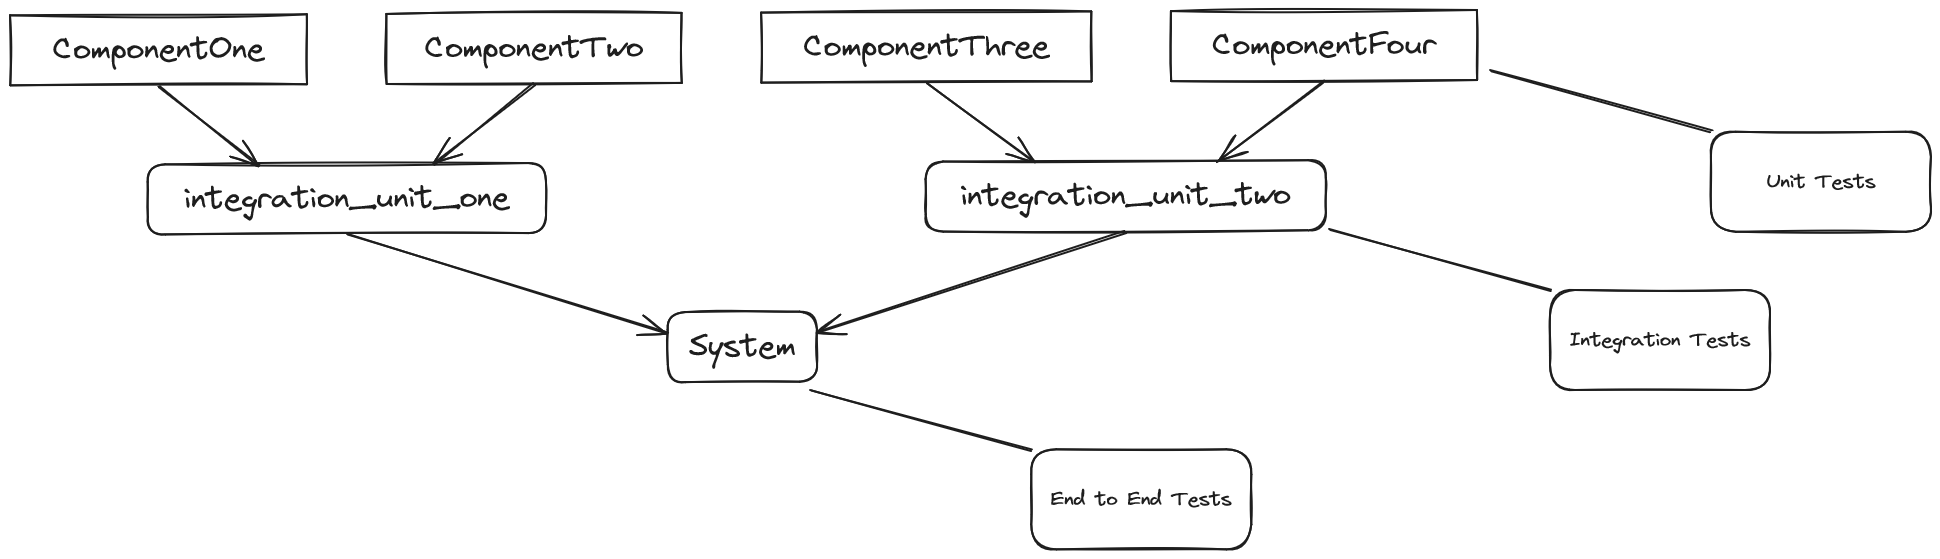
\includegraphics[width=\linewidth]{ModularizedTesting(1).png}

\subsection{The Manual and Automatic Synergy}

The full value of tests is only achieved once the two parts are brought together and that is the essence of
continuous integration. First the computer runs the tests for requested code changes then a reviewer respond with their decision
based on the information gathered by the tests. Thus, the reviewer gets the most amount of information possible to abstract from, code coverage, profiling,
test failures and many more code test reports. Thus, a more thorough analysis than just "this should work because the code looks good" is achieved.
\subsubsection{Regression Tests}

Moreover, the manual review sessions form a feedback loop with the tests. Any bug caught by a review is made into a regression test.
A test that aptly names prevents regresses, that is diving into functionality and bugs that should already be working.

Another importance of regression tests is the mentality that, new changes are tested against old system requirements. This means that tests
for old systems are not just discarded since they can hold important bugs that the new developer did not think of in the replacement system.

\section{The Control}
Now given a thorough testing groundwork, we should ideally be able to construct one big report from the analysis of the code
and based on this analysis, a decision must be made. 
    Do we allow the code to integrate into the shared code base?


\subsection{Version Control Systems}
First, we need to mention how this integration decision is controlled and that in a modern environment through
version control systems. 

This is essential, we want to be able to separate shared code bases that have lesser restrictions on them
and are there for different reasons. Moreover, we must be able to do a rollback in case of mistakes or change of direction
and we want to be able to track who is an appropriate person to ask
for a manual review. For example, Google chooses someone who made changes recently to review a suggested code change \cite{sadowski_modern_2018}.

All this is provided by a modern VCS. \cite{noauthor_version_2018}

\subsection{The Feedback Control}
There is no one size fits all for what decision to make based on the analysis. However, we do have
some software development standards and when deciding what standards we should have we have to look at the
best practices and to what degree we can follow these best practices without sacrificing too much practicality.
Thus, a healthy discussion before the project must be met on the standards of the code base. Once this rule is set, the
team should adhere to these rules when judging test results.

Some best practices are derived from this article \cite{noauthor_standards_nodate}:
\begin{itemize}
    \item Consistent code formatting and style:
    \begin{itemize}
        \item Which industry standard should we follow?
    \end{itemize}
    \item Code readability and documentation:
    \begin{itemize}
        \item Is the code too complex to analyze and debug?
        \item What level is the team on? 
    \end{itemize}
\end{itemize}
\section{A Worked Example: Our Java Calculator}
Now after having discussed the theory let's finish with a practical example, where I and my team used
continuous integration for our product.

\subsection{The CI file}
To do the automated side of the CI process we use git actions. 
It runs the test automatically and
it also generates a report on the tests, this report contains test coverage and results.

https://github.com/Darkfrobozz/inlupp4/blob/main/.github/workflows/makefile.yml

\subsection{A Photo of Test Runs}
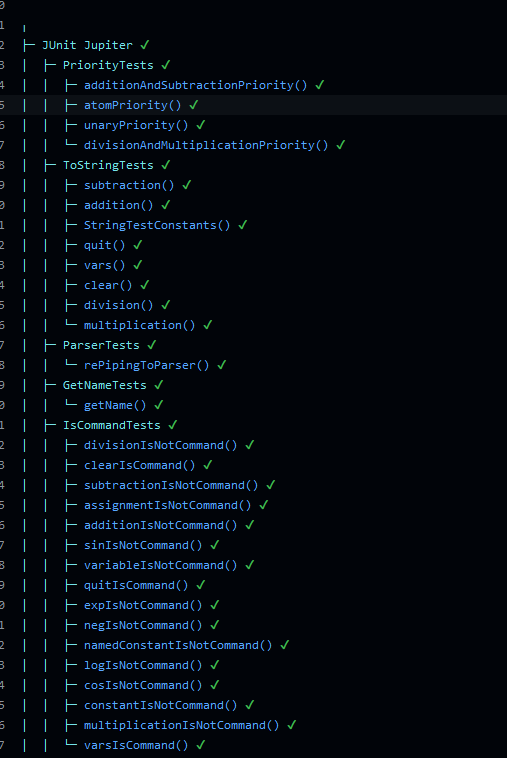
\includegraphics[width=\linewidth]{Screenshot 2023-11-29 161454.png}

\subsection{Protected Branch Control System}
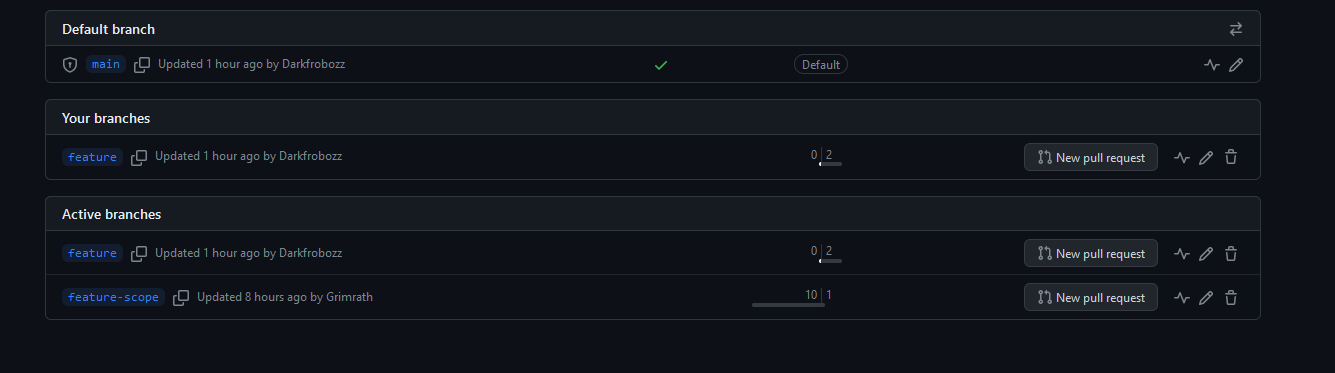
\includegraphics[width=\linewidth]{Screenshot 2023-11-29 161625.png}
Our main branch in this example is protected, so pushing is not allowed to main, one must make a pull request and
the pull request will not go through if no one has reviewed it and if the tests fail.

\section{Conclusion}

This essay is to serve as an introduction to CI, providing the theoretical narrative of
what CI is made of and what is necessary for CI to work correctly.

The essay has highlighted the building blocks of CI that is testing and control. It has explored what
kind of testing is relevant in modern development and how control is decided, of special interest has been the exploration of
the often undervalued role of manual reviews and we can create the correct environment to foster this aspect of CI. This venture is
undertaken because we need to discuss the human side of computer science more. \cite{senthil_behind_2023}
Moreover, the interplay between automated and manual tests has been explored to establish that effective CI is not one or the other
but both since they complement each other not only by filling different roles but also by filling new roles together. 
% Your content goes here
\newpage
\printbibliography
\end{document}